\documentclass[12pt]{article}

% Packages
\usepackage{lmodern}
\usepackage{amsmath} % For mathematical symbols and equations
\usepackage{graphicx} % For including figures
\usepackage{hyperref} % For hyperlinks
\usepackage{listings} % Required for inserting code snippets
\usepackage{xcolor} % Required for custom colors
\usepackage[margin=1in]{geometry}
\usepackage{titling}
\usepackage{setspace}
\usepackage{algorithm}
\usepackage{algorithmic}
\usepackage{enumitem}
\usepackage{float}

\lstset{
    language=R, % Set the language for code snippets to R
    basicstyle=\ttfamily\scriptsize, % Set the font and size for code snippets
    commentstyle=\color{green!60!black}, % Set the color for comments
    stringstyle=\color{orange}, % Set the color for strings
    showstringspaces=false, % Don't show spaces in strings
    breaklines=true, % Allow code to break across lines
    frame=single, % Add a frame around code snippets
    numbers=left, % Add line numbers to code snippets
    numberstyle=\tiny\color{gray}, % Set the style for line numbers
    captionpos=b,
	xleftmargin=0cm,
}

% Title and author
\title{Modeling Canadian Protest Occurrences via Negative Binomial Regression}
\author{Leo Kraushaar \& Ali Hay \\ STAT 413}
\date{\today}

\begin{document}
\onehalfspacing

\begin{titlepage}
  \newcommand{\HRule}{\rule{\linewidth}{0.5mm}}
  \center

  \HRule \\[1cm]
  { \huge \bfseries \thetitle}\\[0.4cm]
  \HRule \\[1cm]

  \Large \thedate\\[5cm]

  \begin{minipage}{1\textwidth}
    \vspace{8cm}
    \begin{flushleft} \large
      \theauthor
    \end{flushleft}

  \end{minipage}
\end{titlepage}

\newpage
\section{Introduction}
For this project, we are working with a dataset containing the number of protests each month from January 2022 until November 2023 in every Canadian province and territory.

Our dataset contained the population size of each province in each month. We also thought it might be interesting to consider the state of the economy in each month over our timeframe, since this could affect how happy individuals are, which could perhaps influence how likely they are to participate in protests. For this reason, we decided to collect some extra data related to economic factors: oil imports (m$^3$), total power generated (MWh), and total retail sales (\$1000).

Our goal in this project is to model the number of protests via a negative binominal regression model, the reasons for which are discussed later. We use our model to create confidence intervals with different bootstrapping methods to determine the most significant model parameters. Finally, we use Monte Carlo simulation to create prediction intervals for the monthly number of protests in each province and territory based on projections for model parameters that we simulated for the year 2030.

Prior to model fitting, we merged all data sources into a single dataset, and performed data cleaning techniques such as granularity reduction and standardization. After fitting our initial model via stepwise selection, we found season, retail, and province to be significant. We compared these results against four bootstrapping methods: resampling, parametric, smooth, and error-sampling. The bootstrap methods were used to create 95\% confidence intervals to identify which of the model parameters were most significant. Lastly, we used Monte Carlo methods to create 95\% prediction intervals for the median number of protests in each Canadian province and territory based on projected retail sales in the year 2030. We created the retail sales projections using historical data, discussed in later sections.
Our primary algorithms and results are included, summarized, and analyzed throughout this report.

\newpage
\section{Model Building}
For this project, we decided to use a negative binomial generalized linear model (glm),which is known to be effective for modeling discrete positive integers (``count data''), the datatype of our response column. The negative binomial model is also known to be resistant to imbalanced expectation/variance ratios (overdispersion), a property notably present in the dataset. We initially fit our model using the predictors \textbf{year, season, province, population, retail, oil, and power}. We standardized the retail predictor before fitting the model, as it was on a much larger scale than the other predictors. We also combined the months into four seasons, as this reduced the standard error of the maximum likelihood estimate of the model's dispersion parameter. Using a stepwise selection method in R, set to minimize model AIC, we created our final model, which contained the significant predictors of season, province, and retail. The final model is shown below, accompanied by relevant scoring metrics and parameter values.

\begin{verbatim}
Call:
glm.nb(formula = protests ~ season + prov + retail, data = data, 
    init.theta = 8.30561596, link = log)

Coefficients:
                              Estimate Std. Error z value Pr(>|z|)    
(Intercept)                    3.68364    0.50985   7.225 5.01e-13 ***
seasonSpring                  -0.06502    0.08264  -0.787 0.431441    
seasonSummer                  -0.55217    0.08629  -6.399 1.57e-10 ***
seasonWinter                  -0.22871    0.08873  -2.578 0.009946 ** 
provBritish Columbia           0.81551    0.16310   5.000 5.73e-07 ***
provManitoba                  -1.91505    0.92108  -2.079 0.037605 *  
provNew Brunswick             -2.62399    1.04409  -2.513 0.011965 *  
provNewfoundland and Labrador -3.06967    1.11340  -2.757 0.005833 ** 
provNorthwest Territories     -5.35839    1.26866  -4.224 2.40e-05 ***
provNova Scotia               -2.41344    0.99351  -2.429 0.015133 *  
provNunavut                   -4.98454    1.26290  -3.947 7.92e-05 ***
provOntario                    5.59695    2.44944   2.285 0.022314 *  
provPrince Edward Island      -4.11279    1.21600  -3.382 0.000719 ***
provQuebec                     2.19032    0.93156   2.351 0.018711 *  
provSaskatchewan              -2.58187    0.94178  -2.741 0.006116 ** 
provYukon                     -4.13848    1.24460  -3.325 0.000884 ***
retail                        -1.85334    1.06448  -1.741 0.081671 .  
---
Signif. codes:  0 ‘***’ 0.001 ‘**’ 0.01 ‘*’ 0.05 ‘.’ 0.1 ‘ ’ 1

(Dispersion parameter for negative binomial(8.3056) family taken to be 1)

    Null deviance: 2091.2  on 298  degrees of freedom
Residual deviance:  349.2  on 282  degrees of freedom
AIC: 1585

Number of Fisher Scoring iterations: 1


              Theta:  8.31 
          Std. Err.:  1.46 

  2 x log-likelihood:  -1548.997 
\end{verbatim}


\begin{figure}[h!]
  \centering
  \fbox{
    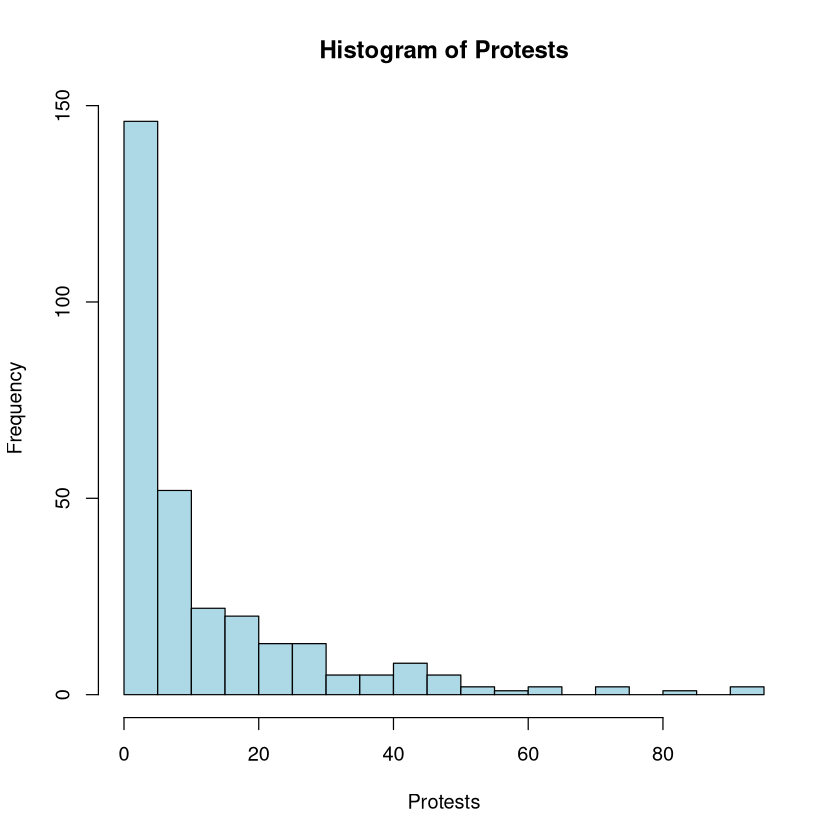
\includegraphics[width=0.5\textwidth]{images/histogram.png}
  }
  \caption{Histogram of Protests}
  \label{fig:your_label}
\end{figure}

\newpage
\section{Bootstrapping for Feature Significance}
\subsection{Resampling Bootstrap}
\subsubsection*{Procedure}
Using $B = 10000$, an algorithm was written to perform a resampling bootstrap on the dataset. On each iteration, a sample of size $n$ (where $n$ was the number of rows in the dataset) was taken with replacement. Using this sample, a new model was fit and the parameter estimates were recorded. Relevant code is shown below.

\vspace{0.5cm}
\begin{lstlisting}[language=R]
resampBoot <- function(df, B) {
	# Get sample size
	n <- nrow(df)
	# Initialize empty dataframe
	params <- c()
	# Initialize progress bar
	bar <- txtProgressBar(min=0, max=B, style=1)
	# Perform B iterations
	for (b in 1:B) {
		# Select a sample of size n
		indices <- sample(1:n, replace = TRUE)
		samp <- df[indices, ]
		# Fit the model with the sample
		boot_model <- glm.nb(protests ~., data=samp, init.theta = 10)
		boot_params <- coef(boot_model)
		params <- rbind(params, boot_params)
		setTxtProgressBar(bar, b)
	}
	close(bar)
	return(params)
}
\end{lstlisting}

\subsubsection*{Results}
We used the resampling bootstrap techniques to test whether there was a significant difference in the mean number of protests in each of the different seasons, with the baseline being fall. The 95\% confidence interval for the spring coefficient did contain 0, but the 95\% confidence intervals for each of the summer and the winter coefficients did not. This tells us that the log mean number of protests in the spring is not significantly different in the spring than the fall, but the log mean number of protests in both the summer and the winter is significantly different than in the fall. Since each of the coefficients for summer and winter are negative and significant, there is strong evidence that protest volume is greater in the fall than in summer and winter.

When using the resampling bootstrap to test for a significant difference in the mean number of protests in each of the different provinces, our baseline province was Alberta. Here, the 95\% confidence intervals for each province and territory showed us that the mean number of protests were significantly different from that of Alberta. British Columbia, Ontario, and Quebec each had a greater mean number of protests than Alberta, whereas the other provinces and territories all had a lower mean number of protests compared to Alberta.
Using the resampling bootstrap, the 95\% confidence interval for the coefficient of retail showed us that retail did not have a significant effect on the mean number of protests.

% latex table generated in R 4.3.3 by xtable 1.8-4 package
% Wed Apr  3 17:34:47 2024
\begin{table}[ht]
\centering
\begin{tabular}{|c|c|c|c|c|c|c|}
  \hline
 & mean & sd & 2.5\% & 50\% & 97.5\% & sig \\ 
  \hline
intercept & 3.66 & 0.53 & 2.70 & 3.64 & 4.77 & TRUE \\ 
  Spr & -0.06 & 0.08 & -0.23 & -0.06 & 0.09 & FALSE \\ 
  Sum & -0.55 & 0.08 & -0.72 & -0.55 & -0.38 & TRUE \\ 
  Win & -0.24 & 0.10 & -0.42 & -0.23 & -0.05 & TRUE \\ 
  BC & 0.82 & 0.14 & 0.55 & 0.82 & 1.09 & TRUE \\ 
  M & -1.89 & 0.93 & -3.85 & -1.85 & -0.18 & TRUE \\ 
  NB & -2.60 & 1.06 & -4.84 & -2.55 & -0.66 & TRUE \\ 
  NL & -3.04 & 1.13 & -5.43 & -2.98 & -0.99 & TRUE \\ 
  NT & -5.40 & 1.37 & -8.20 & -5.34 & -2.94 & TRUE \\ 
  NS & -2.38 & 1.00 & -4.53 & -2.34 & -0.54 & TRUE \\ 
  N & -4.98 & 1.28 & -7.68 & -4.92 & -2.61 & TRUE \\ 
  O & 5.54 & 2.37 & 1.18 & 5.40 & 10.58 & TRUE \\ 
  PEI & -4.10 & 1.23 & -6.73 & -4.04 & -1.82 & TRUE \\ 
  Q & 2.17 & 0.88 & 0.55 & 2.12 & 4.04 & TRUE \\ 
  S & -2.56 & 0.96 & -4.57 & -2.52 & -0.77 & TRUE \\ 
  Y & -4.11 & 1.26 & -6.77 & -4.06 & -1.81 & TRUE \\ 
  retail & -1.83 & 1.04 & -4.05 & -1.77 & 0.08 & FALSE \\ 
   \hline
\end{tabular}
\end{table}


\newpage
\subsection{Parametric Bootstrap}
\subsubsection*{Procedure}
Using $B = 10000$, an algorithm was written to perform a parametric bootstrap on the dataset.

Using the estimated dispersion parameter $\theta \approx 8.31$, each iteration sampled a random vector from a negative binomial distribution with dispersion parameter $\theta$ and mean $\hat y$, where $\hat y$ was the predicted mean value for the corresponding input values.

From the new estimates, a model was fit on each iteration and the parameter estimates were recorded. Relevant code is shown below.
\vspace{0.5cm}
\begin{lstlisting}
conditionalNegBinom <- function(theta, mu) {
    nb_sample <- rnbinom(size=theta, mu=mu, n=1)
    return(nb_sample)
}

paramBoot <- function(B, X, yhat, theta, func) {

    # Initialize empty vector
    params <- c()
    # Iterate B times
    for (b in 1:B) {
        # Simulate NB given means
        sim_y <- sapply(yhat, function(y) func(theta, y))
        # Add to the dataframe
        sim_data <- cbind(X, protests=sim_y)
        # Fit the model to the simulated data
        sim_model <- glm.nb(protests ~., data=sim_data, init.theta = theta)
        # Access the coefficients and store
        parameters <- coef(sim_model)
        params <- rbind(params, parameters)
    }
    return(params)
}
\end{lstlisting}

\subsubsection*{Results}
When using parametric bootstrapping techniques, we came to exactly the same conclusions as we did when using the resampling bootstrapping method. Comparing the widths of these intervals for the seasons with the resampling bootstrap intervals, we found that they were comparable. For the provinces, some of these confidence intervals were wider than the resampling bootstrap intervals, whereas some were narrower. The confidence intervals for retail had a similar standard error, as did most other parameters.

\begin{table}[hbp!]
\centering
\begin{tabular}{|c|c|c|c|c|c|c|}
  \hline
  \textbf{mean} & \textbf{sd} & \textbf{2.5\%} & \textbf{50\%} & \textbf{97.5\%} & \textbf{sig} & \textbf{Z} \\ 
  \hline
3.68 & 0.51 & 2.68 & 3.68 & 4.69 & TRUE & 7.20 \\ 
  -0.07 & 0.08 & -0.23 & -0.07 & 0.10 & FALSE & -0.78 \\ 
  -0.55 & 0.09 & -0.72 & -0.55 & -0.38 & TRUE & -6.35 \\ 
  -0.23 & 0.09 & -0.41 & -0.23 & -0.05 & TRUE & -2.55 \\ 
  0.82 & 0.16 & 0.51 & 0.82 & 1.14 & TRUE & 4.98 \\ 
  -1.92 & 0.92 & -3.75 & -1.91 & -0.11 & TRUE & -2.08 \\ 
  -2.63 & 1.05 & -4.72 & -2.63 & -0.57 & TRUE & -2.51 \\ 
  -3.08 & 1.11 & -5.31 & -3.06 & -0.89 & TRUE & -2.77 \\ 
  -5.41 & 1.27 & -7.92 & -5.39 & -2.91 & TRUE & -4.24 \\ 
  -2.42 & 1.00 & -4.39 & -2.41 & -0.46 & TRUE & -2.43 \\ 
  -5.01 & 1.27 & -7.52 & -5.01 & -2.53 & TRUE & -3.94 \\ 
  5.61 & 2.45 & 0.80 & 5.59 & 10.51 & TRUE & 2.29 \\ 
  -4.13 & 1.22 & -6.54 & -4.12 & -1.73 & TRUE & -3.39 \\ 
  2.20 & 0.93 & 0.36 & 2.19 & 4.07 & TRUE & 2.35 \\ 
  -2.59 & 0.94 & -4.46 & -2.57 & -0.75 & TRUE & -2.74 \\ 
  -4.15 & 1.25 & -6.61 & -4.14 & -1.71 & TRUE & -3.33 \\ 
  -1.86 & 1.07 & -3.98 & -1.85 & 0.23 & FALSE & -1.74 \\ 
   \hline
\end{tabular}
\caption{95\% Confidence Intervals for Model Parameters, Parametric Bootstrap}
\end{table}


\subsection{Smooth Bootstrap}
The smooth bootstrap is not an ``ideal'' method for the given dataset, as only one predictor \textbf{(retail)} was continuous and real-valued. However, results were consistent with other methods, as discussed later.

\subsubsection*{Procedure}
Again using $B = 10000$, an algorithm was written to perform a smooth bootstrap. The \textbf{retail} column was found to have a sample variance of 1, due to the fact that it was standardized prior to model building. A reasonable value for the noise term was chosen, that is, $\frac{1}{\sqrt{n}} \approx 0.05783$. On each iteration, some $\varepsilon_i$ was added to the $i$'th value of retail, where $\varepsilon \sim N(0, 0.05783)$. Using this ``new'' dataset, a model was fit and the paramter estimates were recorded. Relevant code is shown below.

\clearpage
\begin{lstlisting}
addNoise <- function(X) {
    cols <- colnames(X)
    new_X <- X
    for (col in cols) {
        Xi <- X[, col]
        if (class(data[, col]) != "factor") {
            n <- length(Xi)
            S_sq <- var(Xi)
            noise_var <- S_sq / n
            new_X[, col] <- Xi + rnorm(n=n, mean=0, sd=sqrt(noise_var))
        } else {
            new_X[, col] <- Xi
        }
    }
    return(new_X)
}

smoothBoot <- function(X, y, B, noisefunc) {
    # Get sample size
    n <- nrow(X)
    # Initialize empty vector
    params <- c()
    # Initialize progress bar
    pb <- txtProgressBar(min = 0, max = B, style = 3)
    # Perform B iterations
    for (b in 1:B) {
        # Update progress bar
        setTxtProgressBar(pb, b)
        # Get new dataset
        new_X <- noisefunc(X)
        new_data <- data.frame(protests=y, new_X)
        # Fit the model with the simulated data
        smoothboot_model <- glm.nb(protests ~., data=new_data, init.theta = 5)
        boot_params <- coef(smoothboot_model)
        params <- rbind(params, boot_params)
    }
    # Close progress bar
    close(pb)
    return(params)
}
\end{lstlisting}
\subsubsection*{Results}
When using smooth bootstrapping techniques, the results of our 95\% confidence intervals yielded similar conclusions to that of the first two methods, but there were some differences. This method showed us that the mean number of protests was significantly lower in each of the other three seasons than in the fall.
Additionally, using smooth bootstrapping techniques did also lead us to slightly different conclusions when comparing the mean number of protests in each of the provinces and territories. Here we found that each province, except for Manitoba, had a significantly different mean number of protests than Alberta. Again, British Columbia, Ontario and Quebec had more mean protests than Alberta, whereas each of the others had less.
This method also showed us that retail did not have a significant effect on the mean number of protests.

% latex table generated in R 4.3.3 by xtable 1.8-4 package
% Wed Apr  3 19:45:51 2024
\begin{table}[ht]
\centering
\begin{tabular}{rrrrrrlr}
  \hline
 & mean & sd & 2.5\% & 50\% & 97.5\% & sig & abs\_Z \\ 
  \hline
intercept & 3.00 & 0.21 & 2.58 & 3.01 & 3.42 & TRUE & 14.18 \\ 
  seasonSpring & -0.04 & 0.01 & -0.07 & -0.04 & -0.03 & TRUE & -4.59 \\ 
  seasonSummer & -0.55 & 0.01 & -0.56 & -0.55 & -0.54 & TRUE & -80.24 \\ 
  seasonWinter & -0.20 & 0.01 & -0.23 & -0.20 & -0.18 & TRUE & -16.63 \\ 
  BC & 0.67 & 0.05 & 0.57 & 0.67 & 0.76 & TRUE & 13.97 \\ 
  M & -0.67 & 0.39 & -1.43 & -0.68 & 0.10 & FALSE & -1.73 \\ 
  NB & -1.21 & 0.44 & -2.08 & -1.22 & -0.33 & TRUE & -2.76 \\ 
  NL & -1.56 & 0.47 & -2.49 & -1.57 & -0.62 & TRUE & -3.34 \\ 
  NT & -3.68 & 0.52 & -4.70 & -3.68 & -2.63 & TRUE & -7.01 \\ 
  NS & -1.07 & 0.42 & -1.89 & -1.08 & -0.23 & TRUE & -2.57 \\ 
  N & -3.30 & 0.53 & -4.33 & -3.30 & -2.24 & TRUE & -6.27 \\ 
  O & 2.24 & 1.05 & 0.14 & 2.25 & 4.29 & TRUE & 2.14 \\ 
  PEI & -2.47 & 0.51 & -3.48 & -2.48 & -1.45 & TRUE & -4.85 \\ 
  Q & 0.92 & 0.40 & 0.13 & 0.92 & 1.69 & TRUE & 2.32 \\ 
  S & -1.31 & 0.40 & -2.09 & -1.32 & -0.52 & TRUE & -3.32 \\ 
  Y & -2.46 & 0.52 & -3.49 & -2.47 & -1.41 & TRUE & -4.70 \\ 
  retail & -0.39 & 0.45 & -1.29 & -0.40 & 0.52 & FALSE & -0.87 \\ 
   \hline
\end{tabular}
\end{table}


\subsection{Error-Sampling Bootstrap}
\subsubsection*{Procedure}
Another bootstrap method was implemented, in which the error terms from the fitted model were randomly sampled with replacement, and added to the fitted values. Notably, some resulting simulated counts were rounded up to zero in the case where a negative value was produced. This was required both logically; as protests counts cannot be negative, and mathematically; as the negative binomial glm cannot be fit with negative training outputs. As a result, the integrity of the simulated datasets was not assumed to be completely intact, the implications of which are discussed later.

\vspace{0.5cm}
\begin{lstlisting}
epsilonBoot <- function(X, model, B, errors) {

    # Get sample size
    n <- nrow(X)
    # Initialize empty vector
    params <- c()
    # Perform B iterations
    for (b in 1:B) {
        # Get errors
        errs <- sample(errors, size=n, replace=TRUE)
        # Get fitted values
        yhat <- fitted(model)
        # Get simulated y
        ystar <- yhat + errs
        # round up negative values
        ystar <- pmax(rep(0, n), ystar)
        # Turn into DataFrame
        sim_data <- data.frame(protests=ystar, X)
        # Fit the model with the simulated data
        paramboot_model <- glm.nb(protests ~., data=sim_data, init.theta = 5)
        boot_params <- coef(paramboot_model)
        params <- rbind(params, boot_params)
    }
    return(params)
}
\end{lstlisting}
\subsubsection*{Results}
Using the error-sampling bootstrap techniques also produced 95\% confidence intervals that led to slightly different conclusions than the other methods. As with the smooth bootstrapping technique, this method showed us that the mean number of protests was significantly lower in each of the other three seasons than in the fall.
When comparing the mean number of protests in each of the Canadian provinces and territories, we came to the same conclusions using this method as we did with the resampling and parametric bootstraps.
Unlike the other three bootstrapping methods, however, our 95\% confidence interval using the error-sampling bootstrapping showed us that the retail sales did have a significantly negative effect on the mean number of protests. Because of this inconsistency, a natural inference is that the error-sampling bootstrap, at least in this implementation, relies too much on to the validity of the model.

% latex table generated in R 4.3.3 by xtable 1.8-4 package
% Sun Apr  7 20:56:43 2024
\begin{table}[ht]
\centering
\begin{tabular}{rrrrrrlr}
  \hline
 & mean & sd & 2.5\% & 50\% & 97.5\% & sig & abs\_Z \\ 
  \hline
intercept & 3.66 & 0.05 & 3.56 & 3.66 & 3.76 & TRUE & 69.93 \\ 
  seasonSpring & -0.07 & 0.01 & -0.09 & -0.07 & -0.04 & TRUE & -5.54 \\ 
  seasonSummer & -0.56 & 0.02 & -0.59 & -0.56 & -0.53 & TRUE & -34.43 \\ 
  seasonWinter & -0.24 & 0.01 & -0.27 & -0.24 & -0.21 & TRUE & -17.13 \\ 
  BC & 0.82 & 0.02 & 0.78 & 0.82 & 0.86 & TRUE & 38.66 \\ 
  M & -1.89 & 0.09 & -2.07 & -1.89 & -1.71 & TRUE & -20.33 \\ 
  NB & -2.61 & 0.11 & -2.83 & -2.61 & -2.40 & TRUE & -23.98 \\ 
  NL & -3.07 & 0.12 & -3.30 & -3.07 & -2.83 & TRUE & -25.26 \\ 
  NT & -5.20 & 0.28 & -5.80 & -5.18 & -4.70 & TRUE & -18.50 \\ 
  NS & -2.40 & 0.10 & -2.60 & -2.40 & -2.20 & TRUE & -23.24 \\ 
  N & -4.96 & 0.25 & -5.50 & -4.95 & -4.51 & TRUE & -19.51 \\ 
  O & 5.54 & 0.24 & 5.07 & 5.54 & 6.02 & TRUE & 23.00 \\ 
  PEI & -4.16 & 0.18 & -4.51 & -4.15 & -3.83 & TRUE & -23.76 \\ 
  Q & 2.17 & 0.09 & 1.99 & 2.17 & 2.35 & TRUE & 23.50 \\ 
  S & -2.58 & 0.10 & -2.78 & -2.57 & -2.38 & TRUE & -25.32 \\ 
  Y & -4.18 & 0.17 & -4.54 & -4.18 & -3.85 & TRUE & -24.19 \\ 
  retail & -1.82 & 0.10 & -2.03 & -1.82 & -1.62 & TRUE & -17.41 \\ 
   \hline
\end{tabular}
\end{table}


\subsection{Method Comparison}
Using the different Bootstrapping techniques did yield similar conclusions. However, there were a few differences (as mentioned before). We can see from the Z-scores based on the resampling bootstrap that parameters with the highest absolute value of Z-score were summer, followed by British Columbia, then the Northwest Territories, telling us that these were the most significant parameters in our model. The parametric bootstrapping method yielded the same top three most significant parameters as the resampling method. With the smooth bootstrapping method, summer was again the most significant parameter. However it was followed by winter and subsequently British Columbia. Finally, using error-sampling bootstrapping, British Columbia was the most significant parameter, followed by Summer, and then Saskatchewan. Using the error-sampling technique, our Z-scores were much higher in absolute value than the other methods, although smooth bootstrapping did produce some high Z-scores.
Each of our bootstrapping methods produced similar results, with the resampling method and the parametric being the most similar, and the error-sampling method the most different from the other three.

\newpage
\section{Monte Carlo Estimation}
\subsection*{Methods}
Using observations of \textbf{retail} from 2017 to 2022, we fit a linear model predicting the total retail sales using a stepwise selection method using province, year, and season.

We used this model to create 95\% prediction intervals for the retail sales in each province for every month in the year 2030. From this model, we sampled from a $N(\mu, \sigma^2)$ distribution to simulate projected retail values, where $\mu$ was the predicted mean response by the linear model, and $\sigma^2$ was the mean squared error. For each of these projected retail sales, we sampled from our negative binomial model to predict each province's total protests each season. Combining the seasons, we predicted the median number of protests in each Canadian province and territory based on our projected retail sales with 95\% prediction intervals.

\vspace{0.5cm}
\begin{lstlisting}
num_iterations <- 2860
results <- c()

retail_pred_std <- summary(retail_predictor)$sigma
bar <- txtProgressBar(min=0, max=num_iterations, style=1)

for (i in 1:num_iterations) {
    # Get constant values
    blank_data <- data[as.character(data$year) == "2023", ][, c(-3)]
    blank_data$year <- 2030
    retail_preds <- predict.lm(retail_predictor, newdata=blank_data, interval = "prediction")
    pred_means <- retail_preds[, "fit"]
    
    # Predict retail stochastically
    blank_data <- cbind(blank_data, retail_preds)
    blank_data <- as.data.frame(blank_data)
    pred_retails <- rnorm(n=nrow(blank_data), mean=pred_means, sd=retail_pred_std)
    blank_data$retail <- pred_retails
    blank_data[, c("fit", "lwr", "upr")] <- NULL
    blank_data$year <- NULL

    # Predict protests
    blank_data$protests <- predict.glm(model, newdata=blank_data, type="response")
    # Round off to nearest integer
    blank_data$protests <- round(blank_data$protests)
    rownames(blank_data) <- NULL
    results <- rbind(results, blank_data)
    setTxtProgressBar(bar, i)
}
close(bar)
\end{lstlisting}

\subsection*{Results}
Here we compare 95\% Monte Carlo prediction intervals with the observed number of protests in each province during the year 2023. Each of the confidence intervals, except for Quebec and Ontario, are entirely below the observed number of protests in 2023. This is to be expected as total retail sales have a negative association with number of protests, which we can see from the negative estimate of the parameter, meaning that as the total retail sales increase, the number of protests is expected to decrease. In 2030, it is expected that the total retail sales will increase, so this increase in retail sales explains the typical predicted decrease in protests. The lack of decrease in protests in Ontario and Quebec could have been due to random variation in the number of protests in 2023. For example, Ontario and Quebec may have had a large number of protests in that year.


\begin{table}[H]
\centering
\begin{tabular}{|l|c|c|c|c|c|c|}
  \hline
\textbf{prov} & \textbf{2023} & \textbf{2.5\%} & \textbf{50\%} & \textbf{97.5\%} & \textbf{pred.effect} & \textbf{sig.effect} \\  
  \hline
Alberta & 139 & 103 & 116 & 131 & dec. & Y \\ 
  British Columbia & 284 & 193 & 218 & 245 & dec. & Y \\ 
  Manitoba & 118 & 63 & 71 & 81 & dec. & Y \\ 
  New Brunswick &  61 & 37 & 42 & 48 & dec. & Y \\ 
  Newfoundland \& Labrador &  61 & 26 & 30 & 34 & dec. & Y \\ 
  Northwest Territories &   6 & 0 & 0 & 2 & dec. & Y \\ 
  Nova Scotia &  85 & 43 & 48 & 55 & dec. & Y \\ 
  Nunavut &  11 & 3 & 5 & 7 & dec. & Y \\ 
  Ontario & 627 & 668 & 755 & 849 & inc. & Y \\ 
  Prince Edward Island &  29 & 11 & 12 & 15 & dec. & Y \\ 
  Quebec & 270 & 250 & 282 & 317 & inc. & N \\ 
  Saskatchewan &  56 & 33 & 38 & 43 & dec. & Y \\ 
  Yukon &  18 & 11 & 12 & 15 & dec. & Y \\ 
   \hline
\end{tabular}
\caption{95\% Prediction Intervals for Total Yearly Protests by Province, 2030} 
\end{table}


\newpage
\section{Conclusion}
For this project, we fit a negative binomial Generalized Linear Regression Model including the predictors season, retail, and province. We used this model to perform resampling bootstrapping, parametric bootstrapping, smooth bootstrapping and error-sampling bootstrapping to create 95\% confidence intervals. In all four cases, summer and British Columbia were in the top three most significant parameters. Finally, we created projections for retail sales in 2030 and used these to create 95\% Monte Carlo prediction intervals for the median number of protests in each Canadian province and territory. These projected increases in sales led to decreased predictions for the number of protests in each province, except for the two in our model with the largest positive parameter estimates, Ontario and Quebec.
Overall, using methods learned in STAT 413, we were able to come to interesting conclusions regarding Canadian protests.

\newpage
\section*{Bibliography}

\hspace{0.6cm}Hilbe, J. M. (2011). Negative binomial regression: modeling. In Negative Binomial Regression (pp. 221-283). Cambridge University Press.
\vspace{0.5cm}

Statistics Canada. (2024, March 4). Historical (real-time) releases of monthly retail trade, sales (x 1,000) [Data table]. doi.org/10.25318/2010008101-eng
\vspace{0.5cm}

Statistics Canada. (2024, April 2). Electric power generation, monthly receipts, deliveries and availability [Data table]. doi.org/10.25318/2510001601-eng
\vspace{0.5cm}

Statistics Canada. (2020, February 19). Monthly Oil and Other Liquid Petroleum Products Pipeline Survey (MOPS).

\end{document}